\section{Training operators to assemble a starter motor using an immersive HMI}\label{sec:training}

Small parts assembly of flexible components is a very challenging task to automate given the advanced sensing and gripping technologies that it requires. As such, currently it is more cost effective to have cooperative assembly lines in which humans perform the tasks that require robust perception, adaptive grasping and high level cognition while the robots do the remaining tasks.

In the next sections, we will present the application of our immersive training system for the assembly of a starter motor. This is a representative use case of small parts assembly given its diversity of operations and components. Moreover, since it has flexible parts (rubbers, wires, springs), it would be a prime candidate for a collaborative assembly line, in which besides teaching, our immersive \gls{hmi} system could also be used to coordinate the assembly process between the operator and the robotic system.



\subsection{Testing platform}

Our immersive teaching system was developed as a \gls{ros}\footnote{\url{http://www.ros.org}} package for fast integration into robotic workstations and relies on the Gazebo simulator for 3D rendering and the \gls{pcl} for 3D perception. It was tested with a BenQ W1070 \gls{dlp} projector for overlying the teaching information into the environment, an Asus Xtion Pro Live structured light 3D sensor for 6 \gls{dof} pose estimation of objects and a Kinect 2 \gls{tof} 3D sensor for the user interaction analysis. In \cref{fig:hardware} it can be seen the work area and the hardware disposition (in the right image the projector is on the top right, the Kinect 2 is on the left, the Asus Xtion is below the projector and the David Laser 3D structured light system camera is at the top).

\begin{figure}[ht]
	\centering
	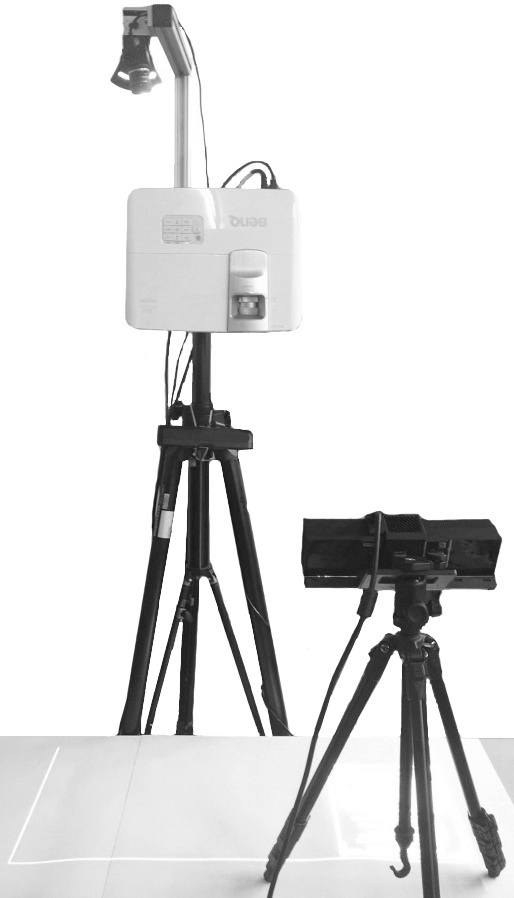
\includegraphics[height=.24\textheight]{hardware-front}
	\hspace{2em}
	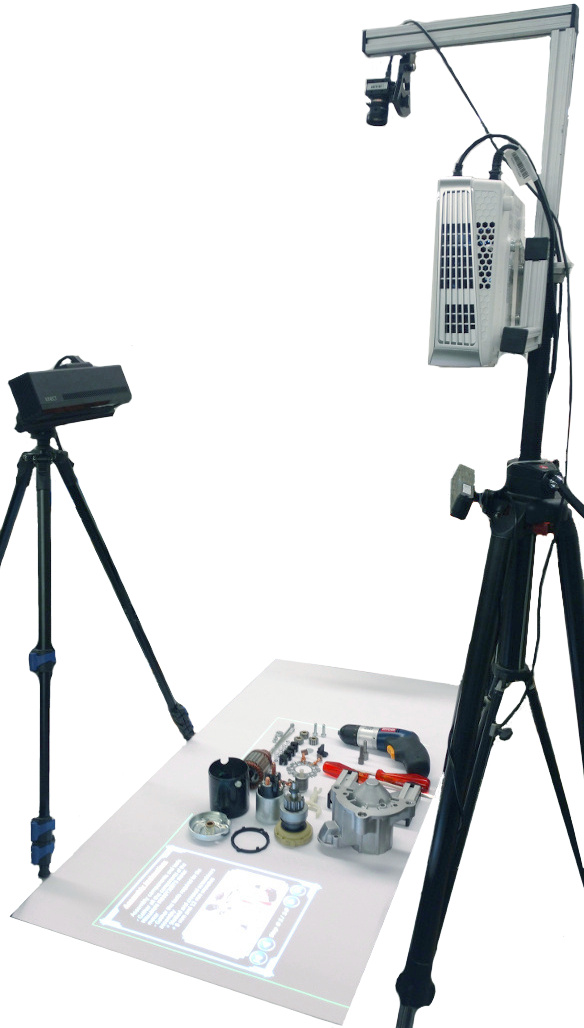
\includegraphics[height=.24\textheight]{hardware-side}
	\caption{Hardware setup}
	\label{fig:hardware}
\end{figure}



\subsection{Training session}

The training session started by gathering all the assembly parts and the required tools for performing the starter motor assembly (shown in \cref{fig:assembly-parts}). Then using the proposed immersive teaching system, the operator read the instructions, watched the videos and navigated through the assembly steps using the projected interaction buttons (displayed in \cref{fig:interaction-pause,fig:interaction-next,fig:interaction-seek}) until it completed the assembly process. Namely, the operator started by assembling the brushes into the brush holder (seen in \cref{fig:step2}) and then bended the braided cables for ensuring that the brushes were perpendicular to the armature, that was assembled later on (shown in \cref{fig:step3}). These kind of operations that involve flexible parts with cables and rubbers are very hard to automate with robotic manipulators, and as such, are the ideal candidate for being assigned to operators. On the other hand, assembly steps that deal with large and rigid parts can be delegated to robots, which is the case of step 4 (displayed in \cref{fig:step4}), in which the operator assembled the rear bracket and attached the large cylindrical yoke. This way, the operator could be performing steps 5 to 8 in parallel, which involve the lower section of the starter motor while the robot was finishing the assembly of the top section. The step 5 included the placement of the large bottom bracket on top of a fixture for holding it vertically, followed by the assembly of the clutch and shift lever (presented in \cref{fig:step5}). Then, step 6 included the assembly of the 3 planetary gears (shown in \cref{fig:step6}) while in step 7 the plunger and several isolation rubbers were installed (displayed in \cref{fig:step7}). Later on, the plunger spring and its magnetic switch were attached to the lower section of the starter motor (as seen in \cref{fig:step8}). Finally, the lower and upper section of the starter motor were assembled together (presented in \cref{fig:step9}), followed by a visual inspection of the assembled product (seen in \cref{fig:step10,fig:projection-mapping-2,fig:projection-mapping-3}).

For helping the operator during the final inspection phase, the proposed \gls{sar} system estimated the 6 \gls{dof} pose of the starter motor and then projected its expected outline on top of it. The main purpose of this final stage was to test the accuracy of the proposed \gls{sar} system. Namely, to evaluate if the proposed \gls{sar} system was able to achieve a good overlap between the physical and virtual objects. This would implicitly confirm that the approach proposed to model the 3D camera within Gazebo along with the subsystems that influence the rendering of the starter motor outline (calibration of the projector, cameras and 3D sensors along with 6 \gls{dof} pose estimator) were suitable for achieving a usable \gls{sar} system. Looking at \cref{fig:step10,fig:projection-mapping-2,fig:projection-mapping-3}, the overall overlap error seems to be below 2 mm, making the proposed \gls{sar} system ready to be applied to other use cases and be used as a starting point for developers wanting to incorporate \gls{sar} into their products, such as cooperative workstations in which operators and robots work side by side.

\begin{figure}[H]
	\begin{floatrow}[2]
		\ffigbox[\FBwidth]
		{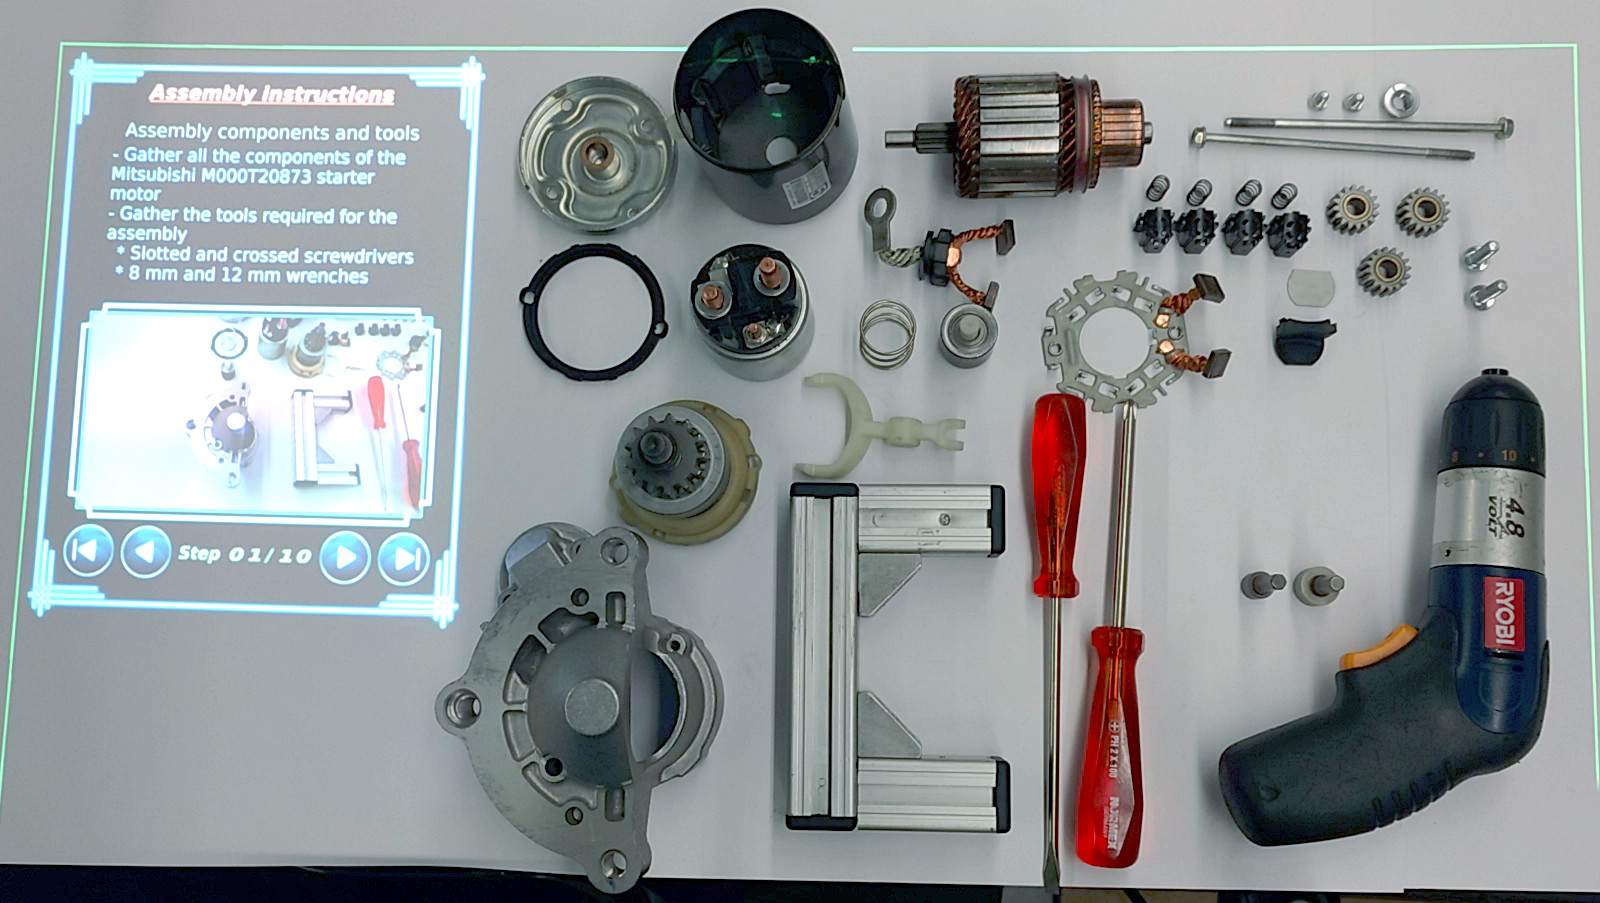
\includegraphics[height=.103\textheight]{steps/1}}
		{\caption{Step 1 - starter motor parts and assembly tools}\label{fig:assembly-parts}}
		\ffigbox[\FBwidth]
		{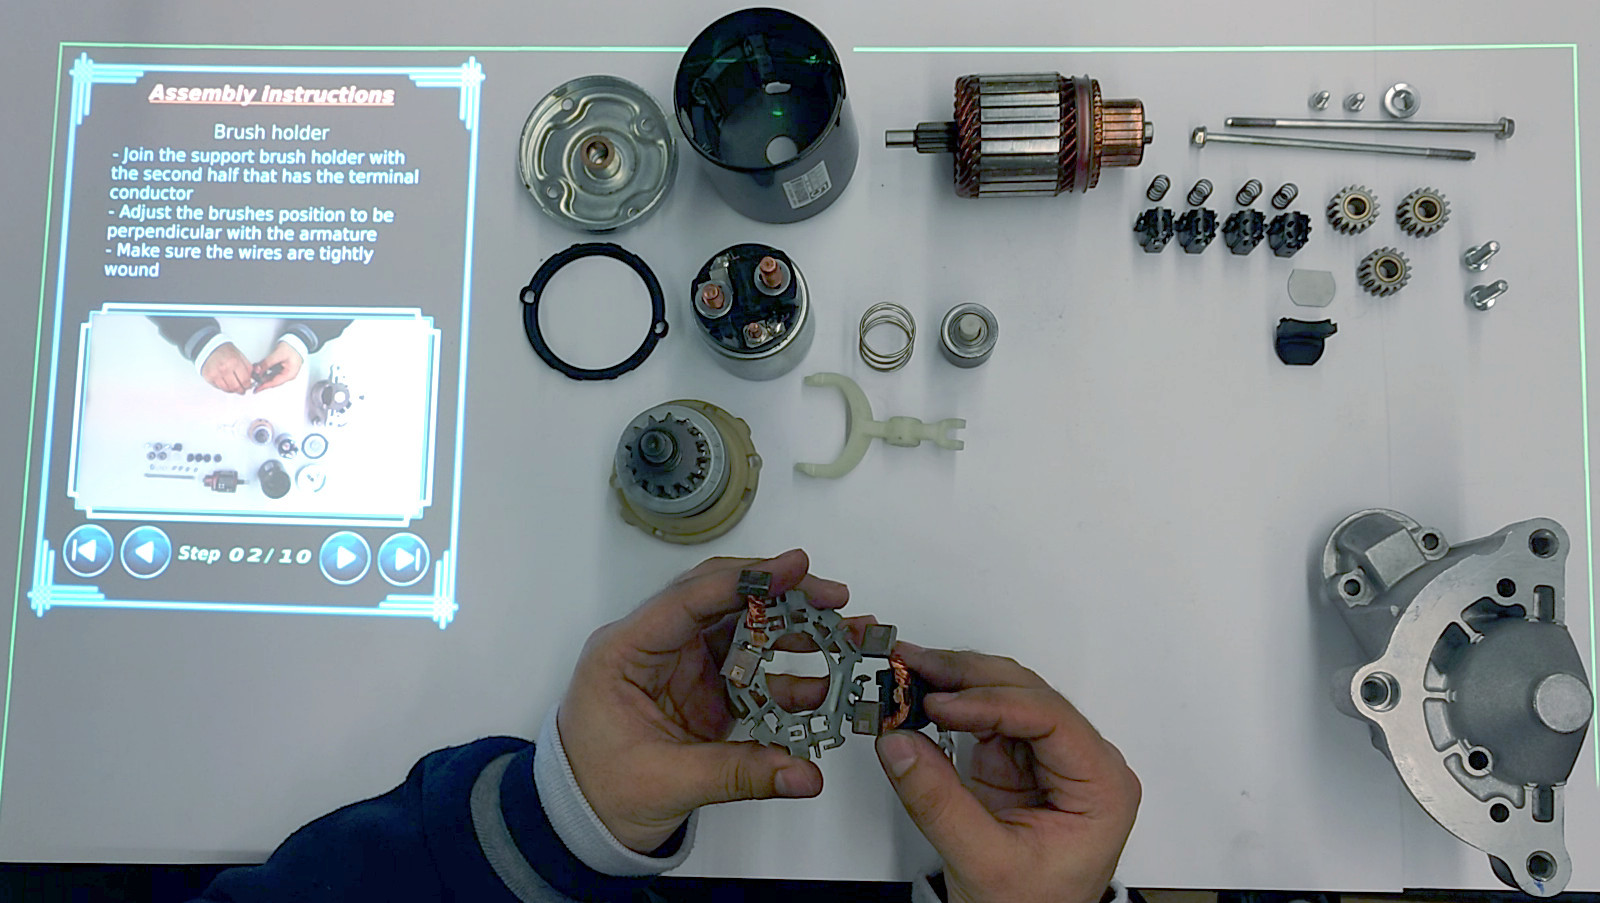
\includegraphics[height=.103\textheight]{steps/2}}
		{\caption{Step 2 - assembly of the brush holder}\label{fig:step2}}
	\end{floatrow}
\end{figure}

\begin{figure}[H]
	\begin{floatrow}[2]
		\ffigbox[\FBwidth]
		{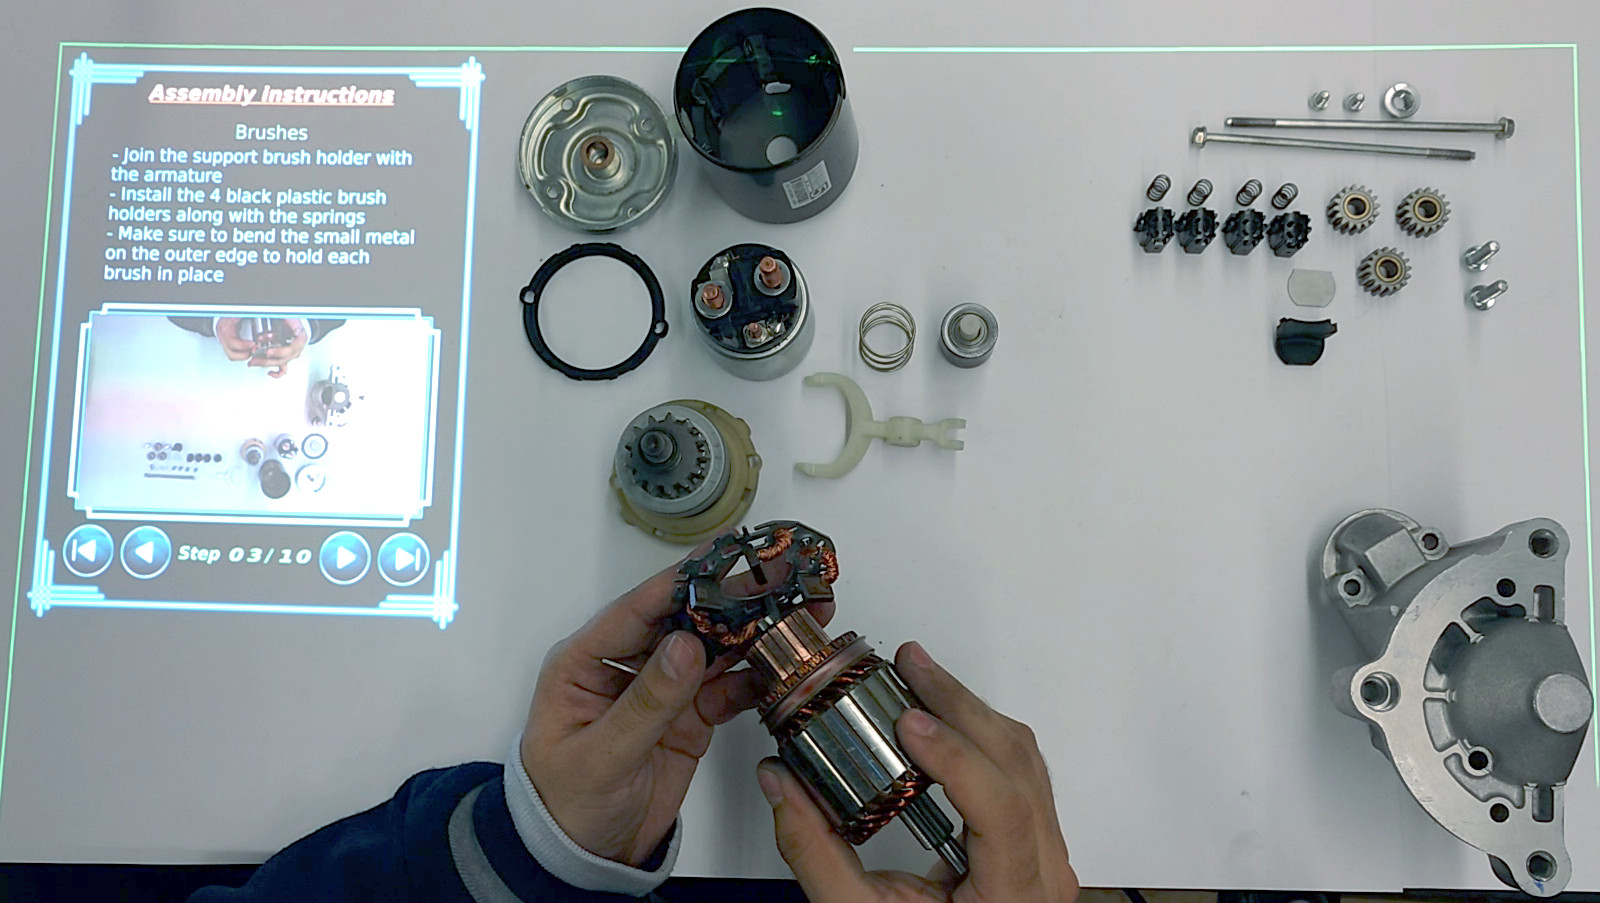
\includegraphics[height=.103\textheight]{steps/3}}
		{\caption{Step 3 - assembly of the brushes into the armature}\label{fig:step3}}
		\ffigbox[\FBwidth]
		{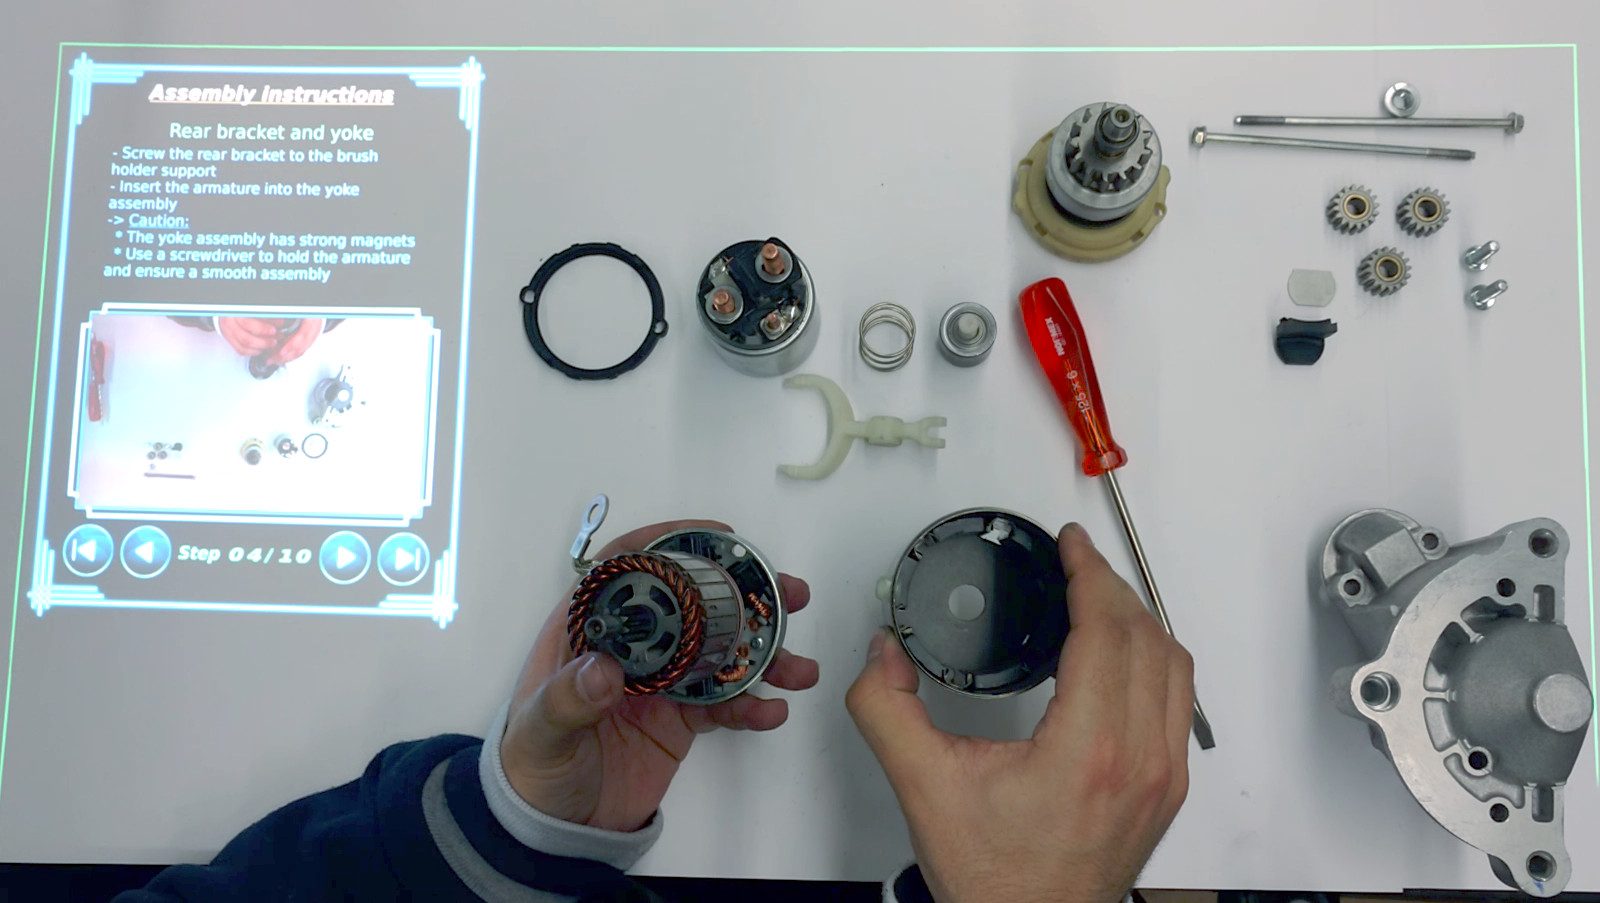
\includegraphics[height=.103\textheight]{steps/4}}
		{\caption{Step 4 - assembly of the rear bracket and yoke}\label{fig:step4}}
	\end{floatrow}
\end{figure}

\begin{figure}[H]
	\begin{floatrow}[2]
		\ffigbox[\FBwidth]
		{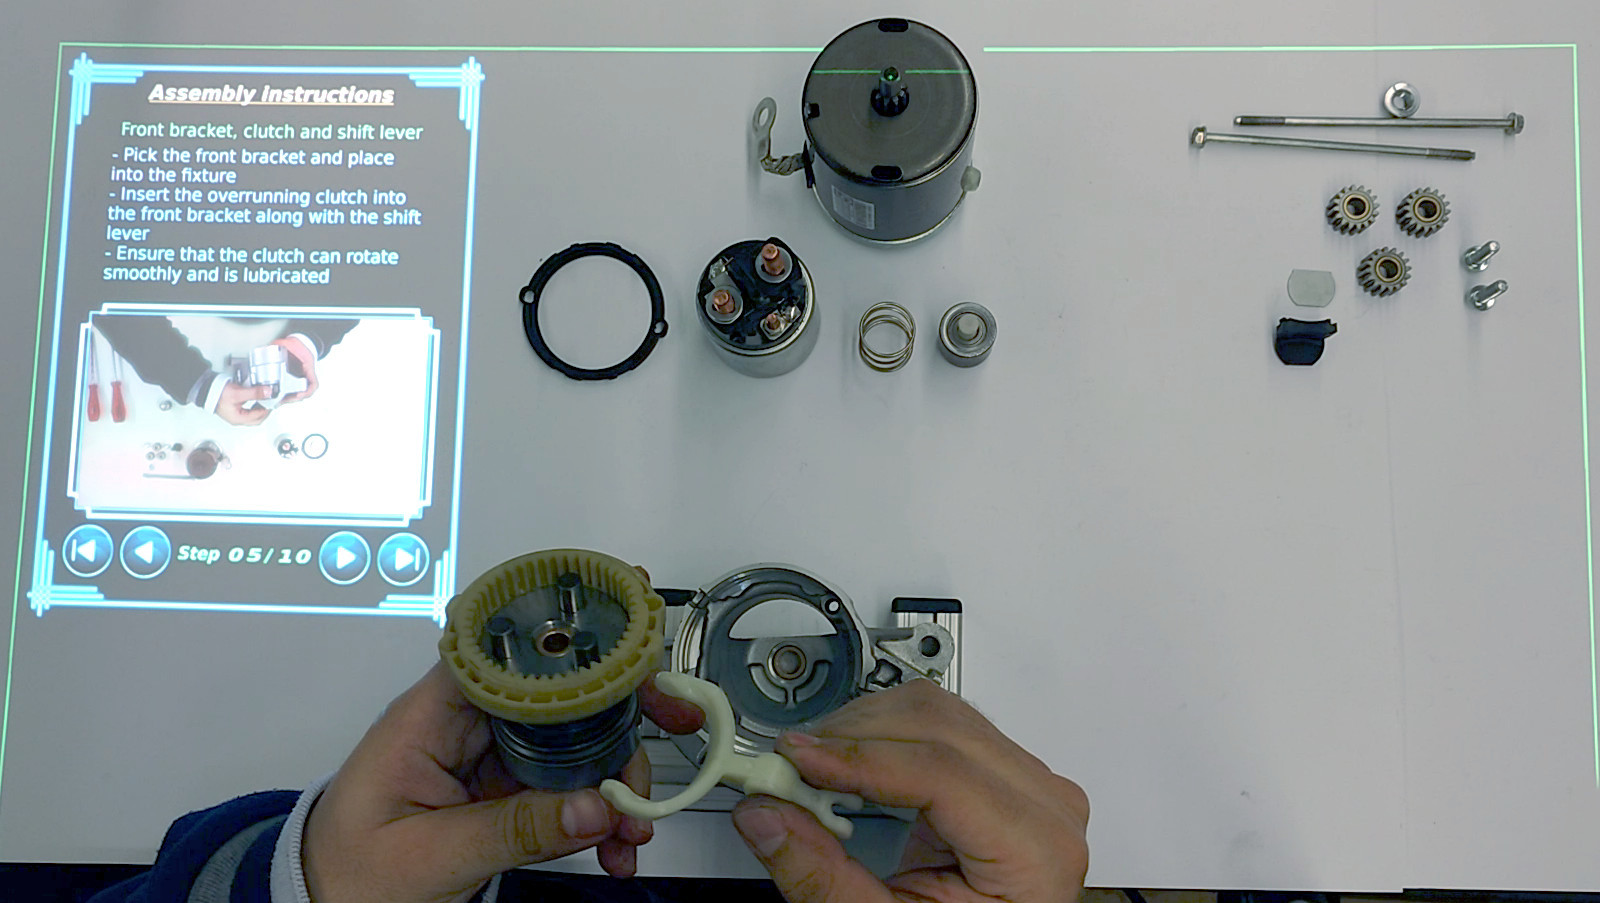
\includegraphics[height=.103\textheight]{steps/5}}
		{\caption{Step 5 - assembly of the front bracket, clutch and shift lever}\label{fig:step5}}
		\ffigbox[\FBwidth]
		{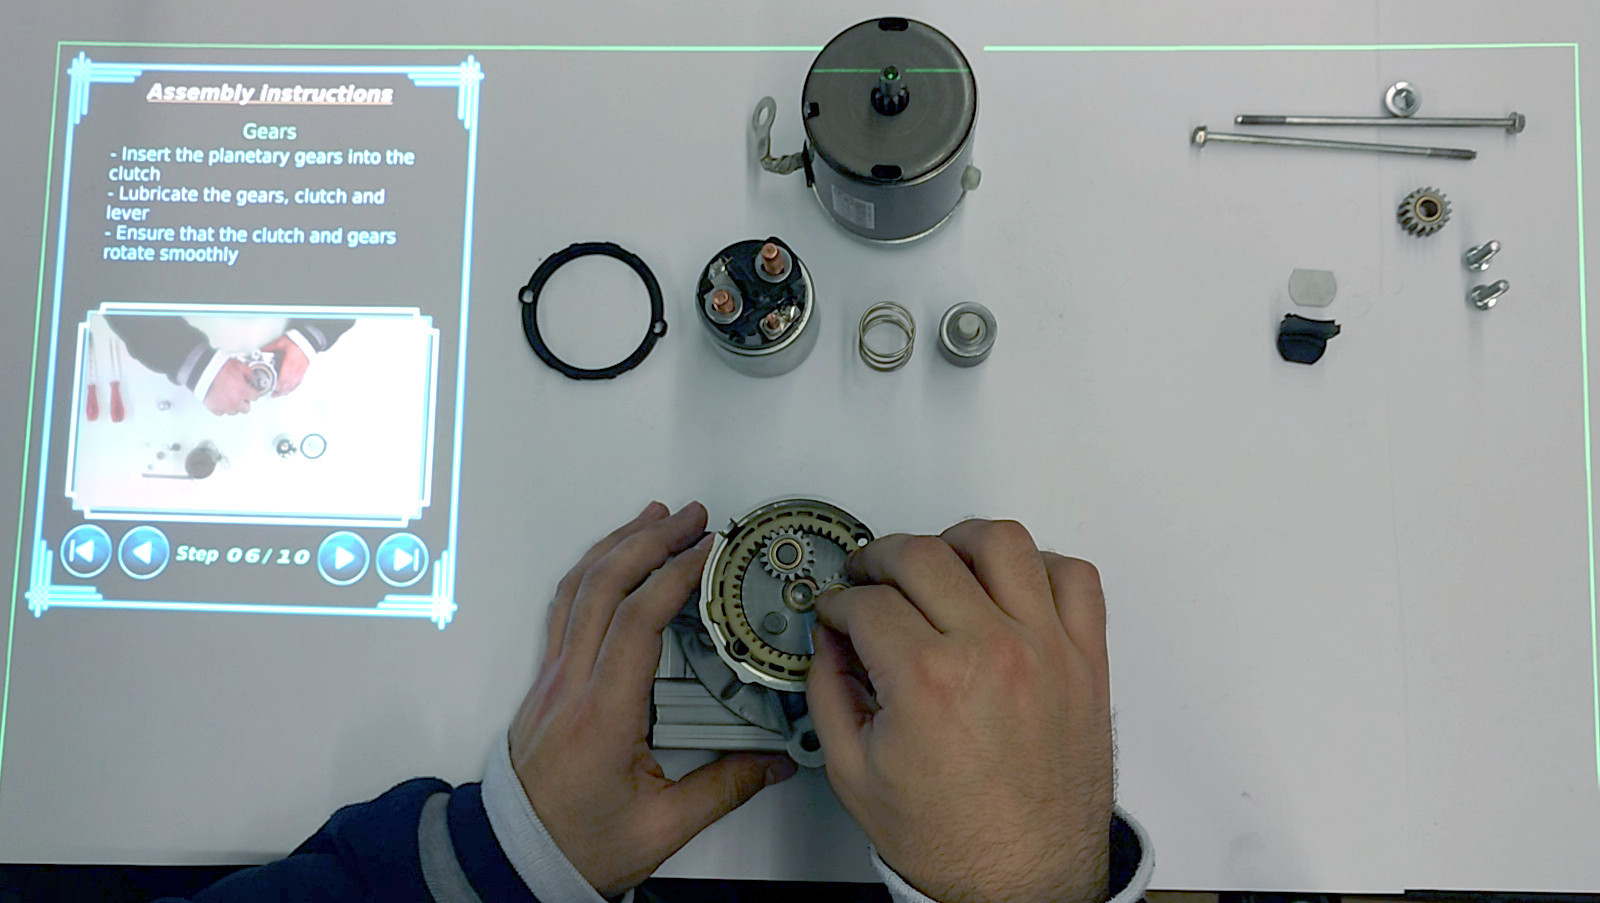
\includegraphics[height=.103\textheight]{steps/6}}
		{\caption{Step 6 - assembly of the planetary gears}\label{fig:step6}}
	\end{floatrow}
\end{figure}

\begin{figure}[H]
	\begin{floatrow}[2]
		\ffigbox[\FBwidth]
		{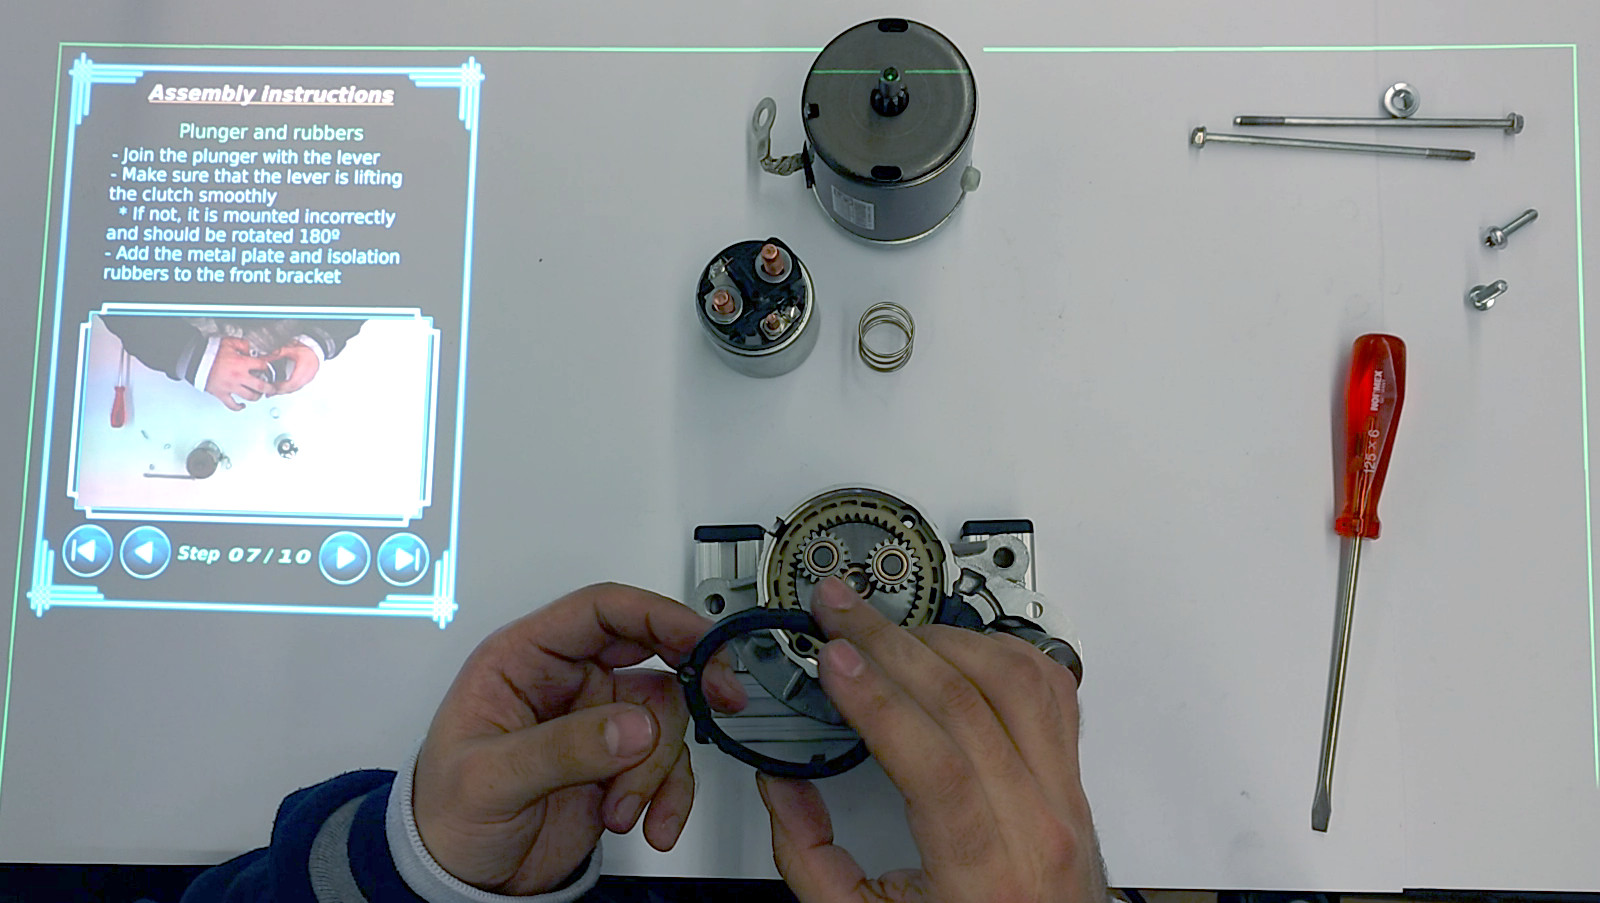
\includegraphics[height=.103\textheight]{steps/7}}
		{\caption{Step 7 - assembly of the plunger and rubbers}\label{fig:step7}}
		\ffigbox[\FBwidth]
		{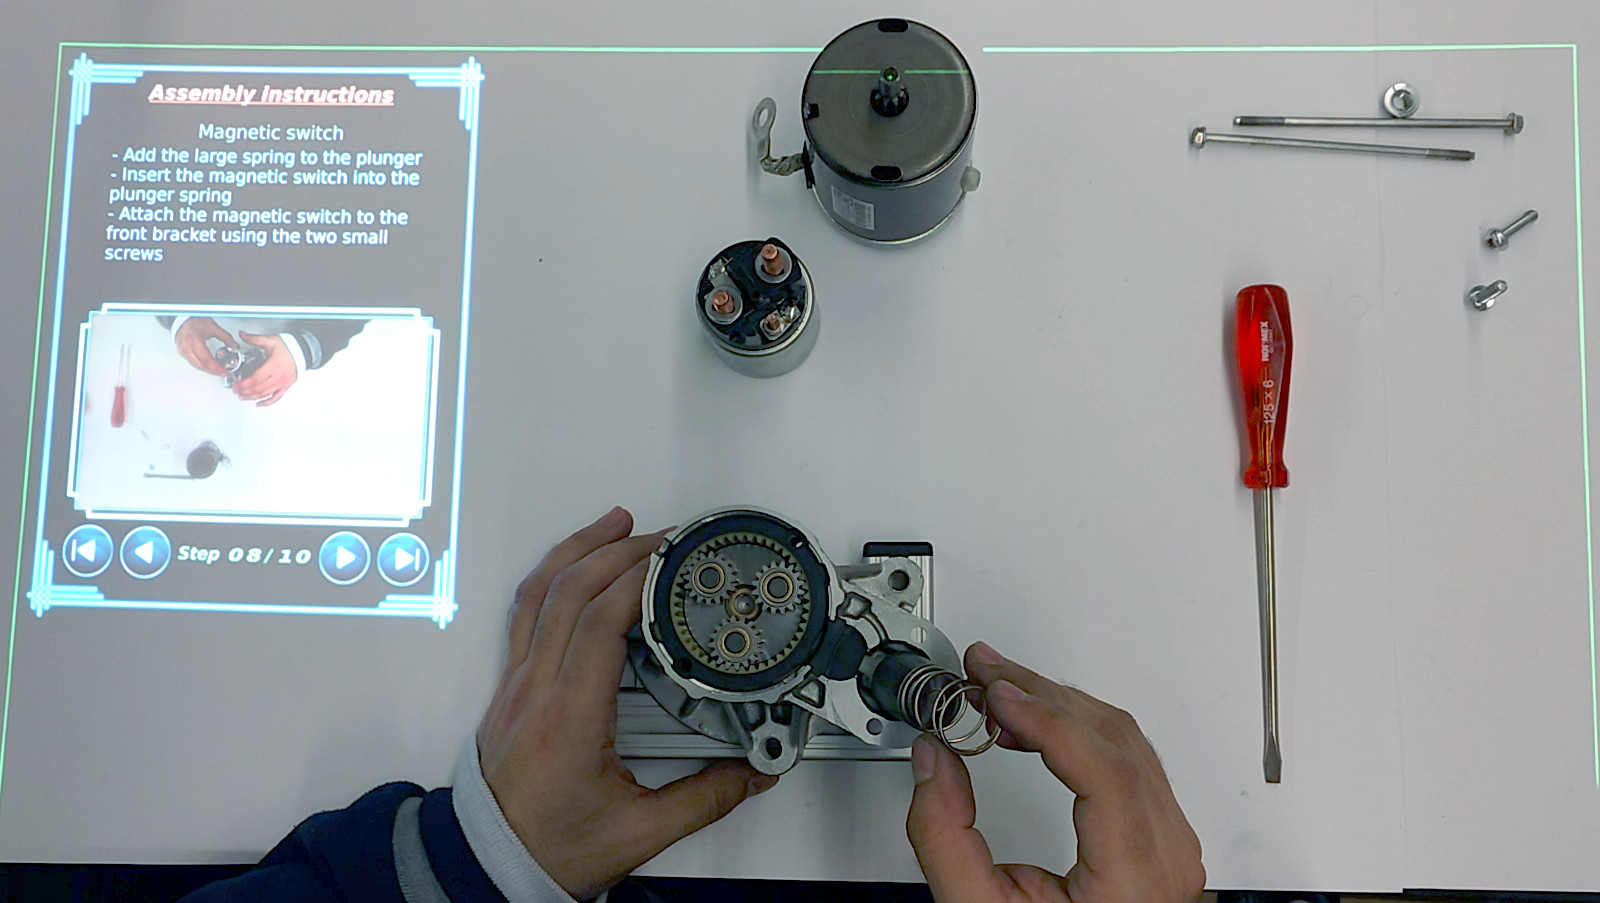
\includegraphics[height=.103\textheight]{steps/8}}
		{\caption{Step 8 - assembly of the plunger spring and magnetic switch}\label{fig:step8}}
	\end{floatrow}
\end{figure}

\begin{figure}[H]
	\begin{floatrow}[2]
		\ffigbox[\FBwidth]
		{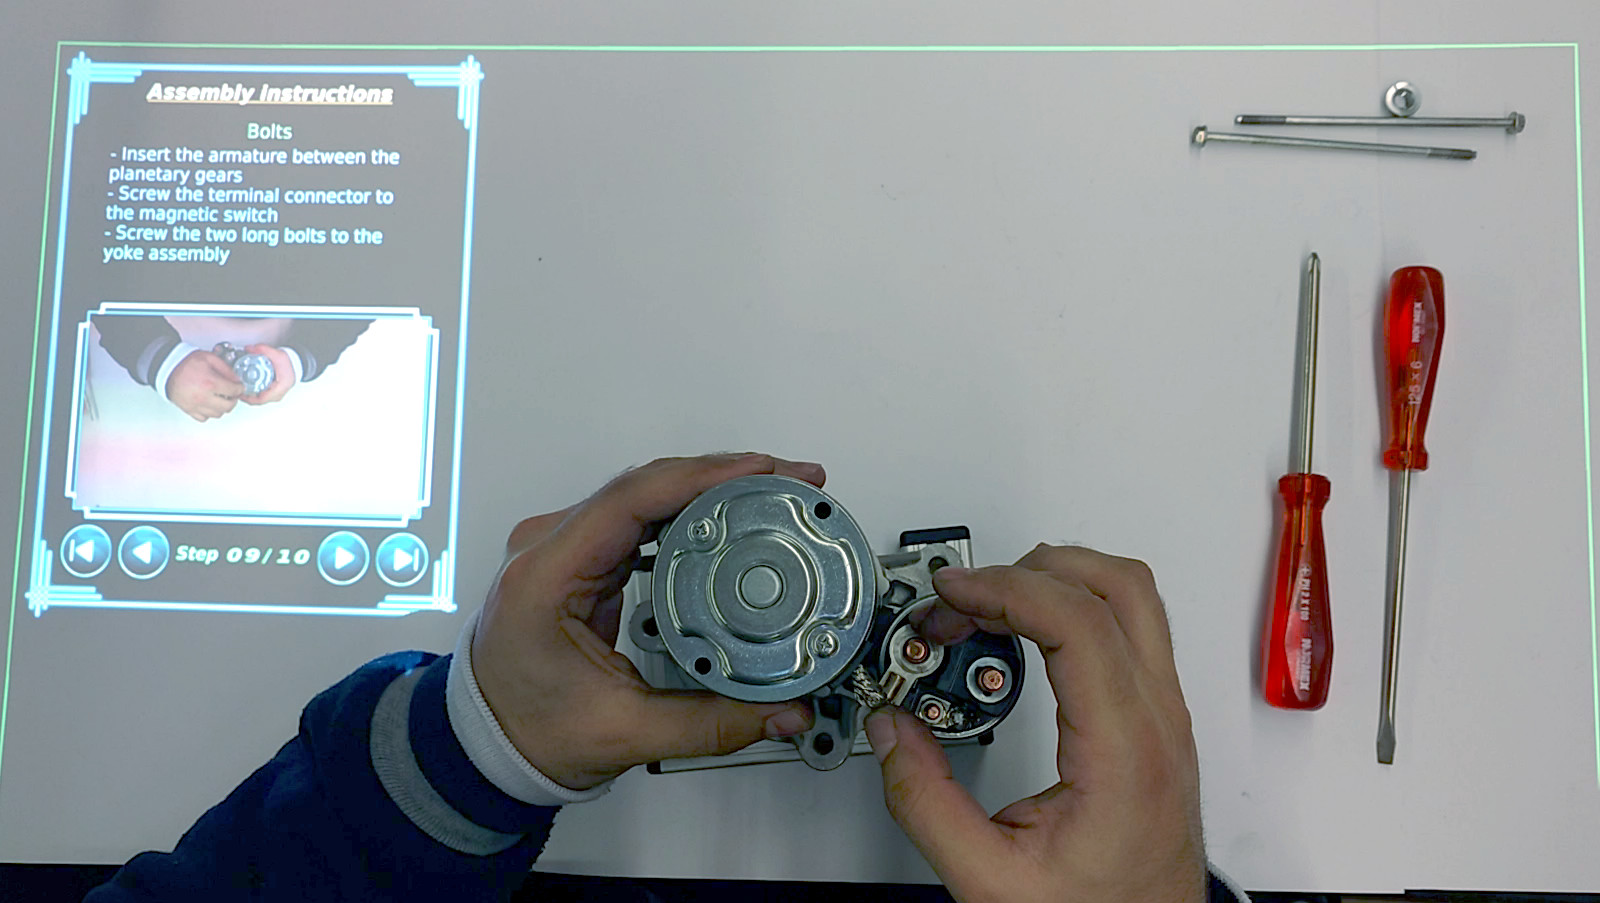
\includegraphics[height=.103\textheight]{steps/9}}
		{\caption{Step 9 - assembly of the armature and its bolts}\label{fig:step9}}
		\ffigbox[\FBwidth]
		{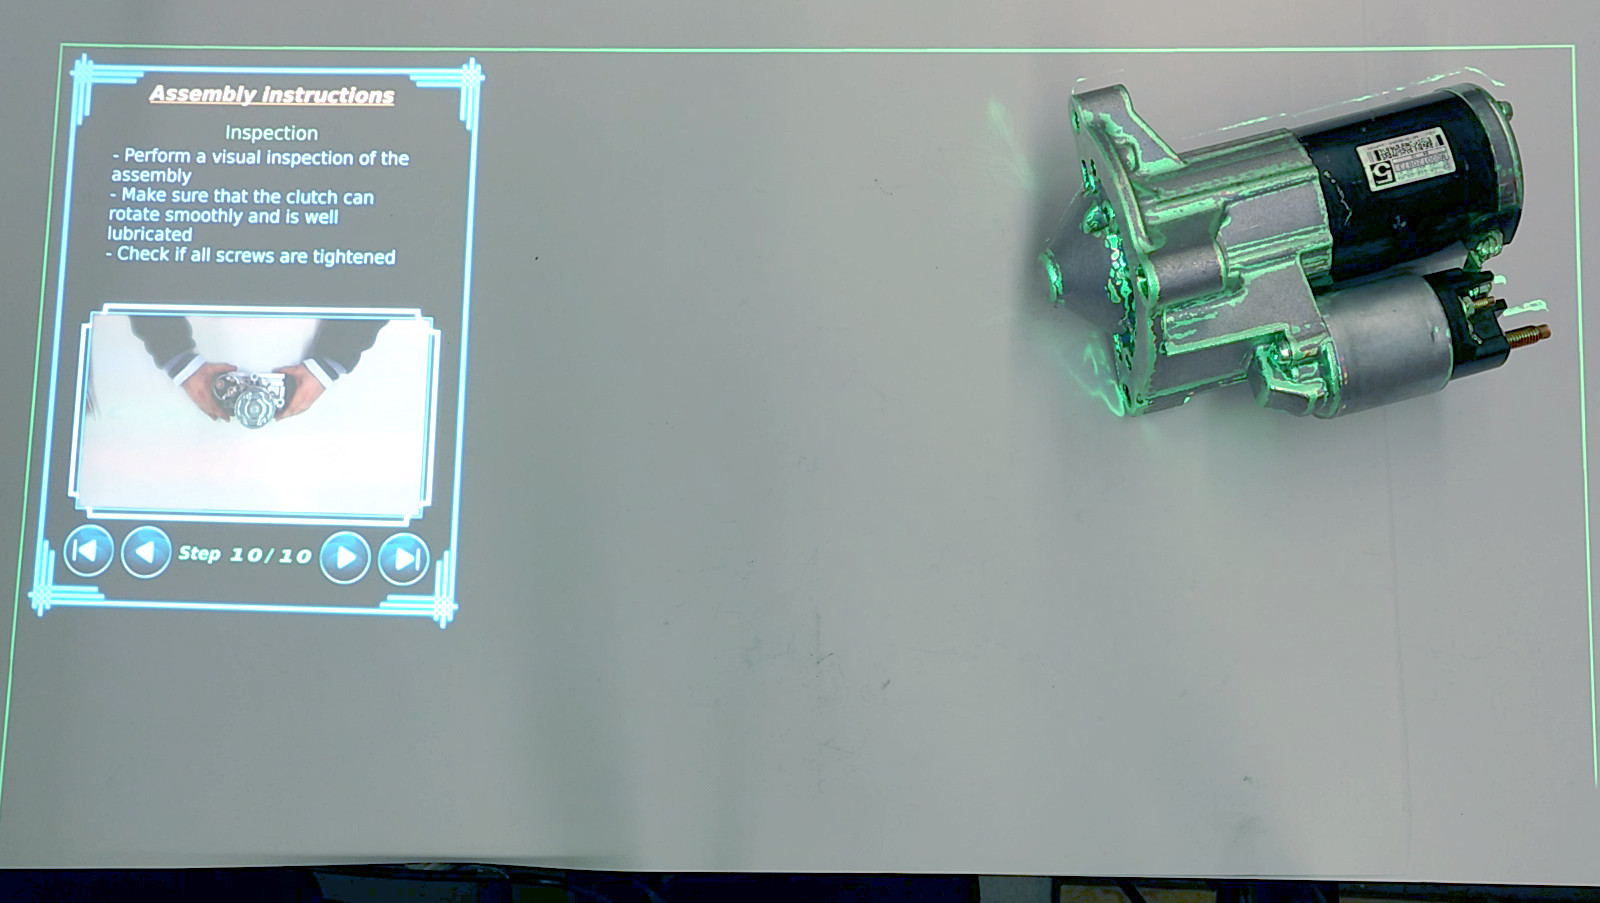
\includegraphics[height=.103\textheight]{steps/10}}
		{\caption{Step 10 - visual inspection of the assembled product}\label{fig:step10}}
	\end{floatrow}
\end{figure}

\begin{figure}[H]
	\begin{floatrow}[2]
		\ffigbox[\FBwidth]
		{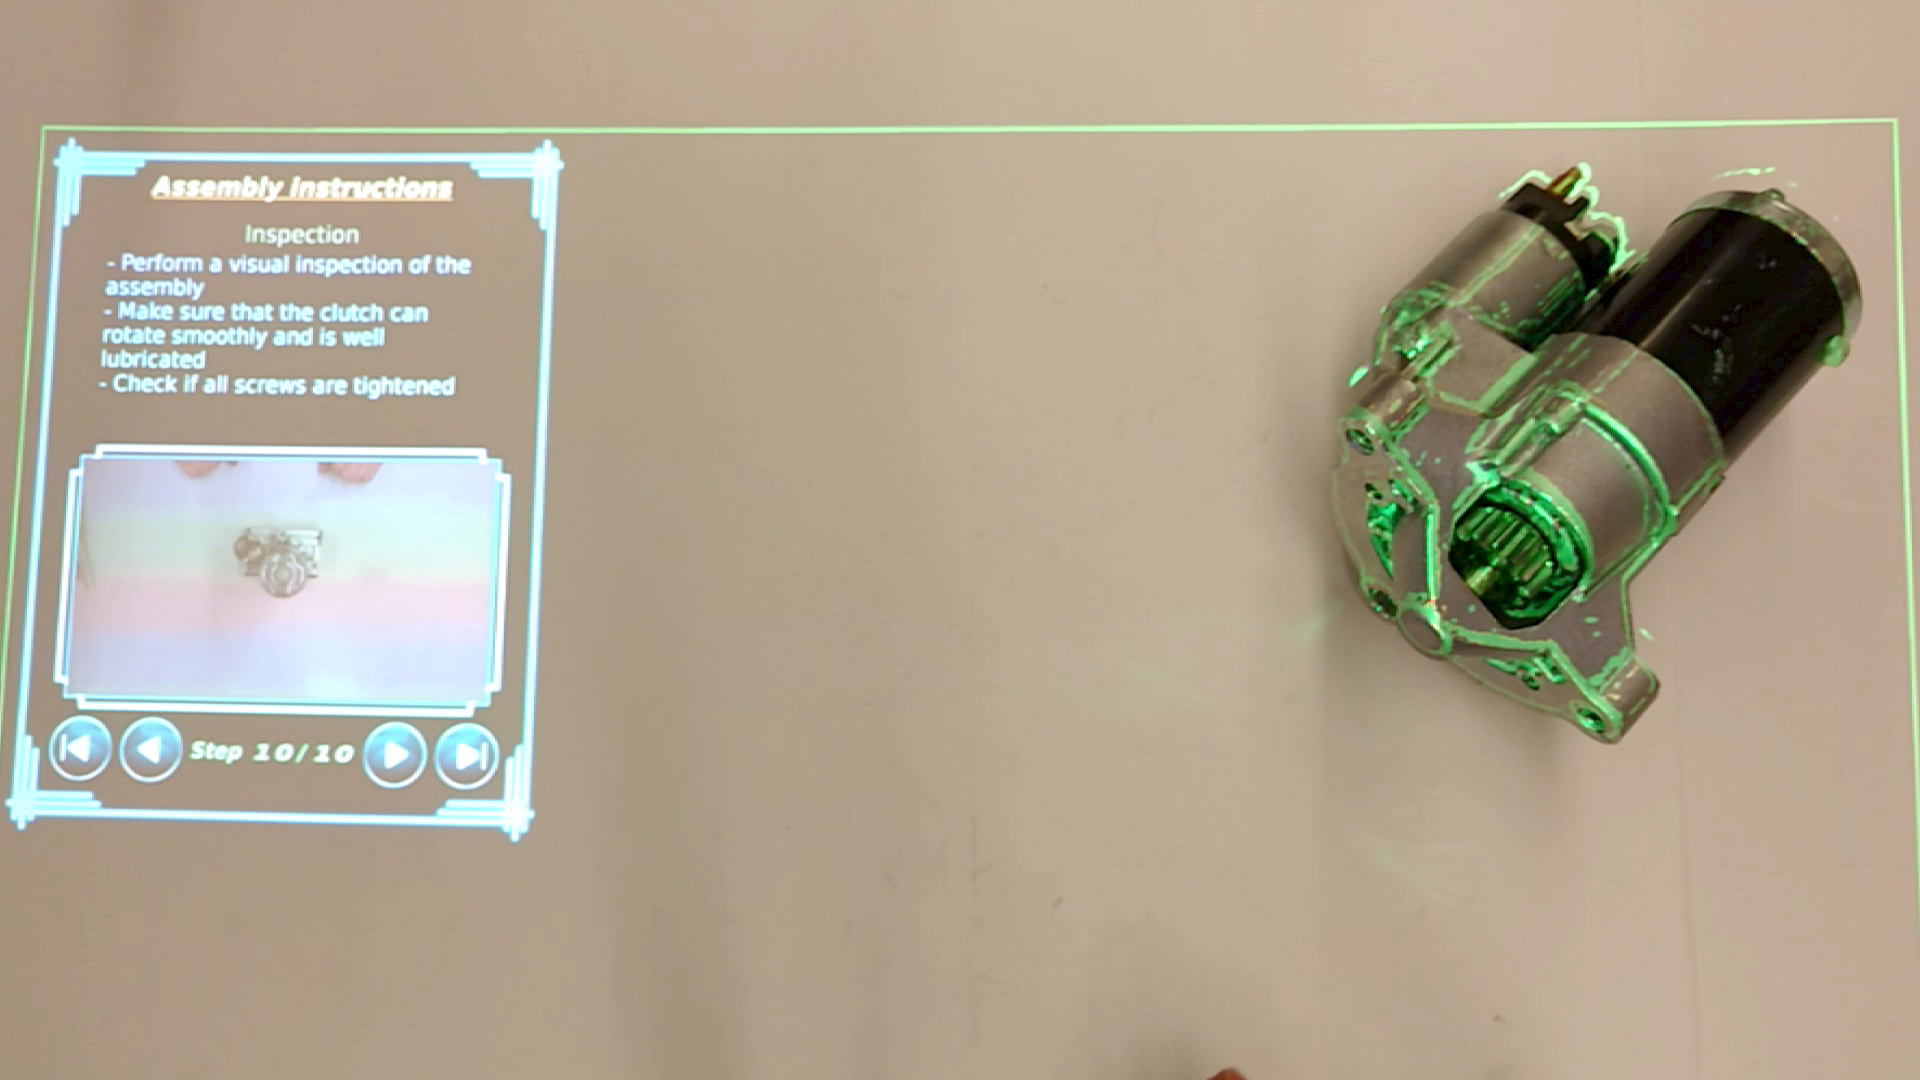
\includegraphics[height=.117\textheight]{projection-mapping-2}}
		{\caption{Detailed view of the validation projection for the inspection phase}\label{fig:projection-mapping-2}}
		\ffigbox[\FBwidth]
		{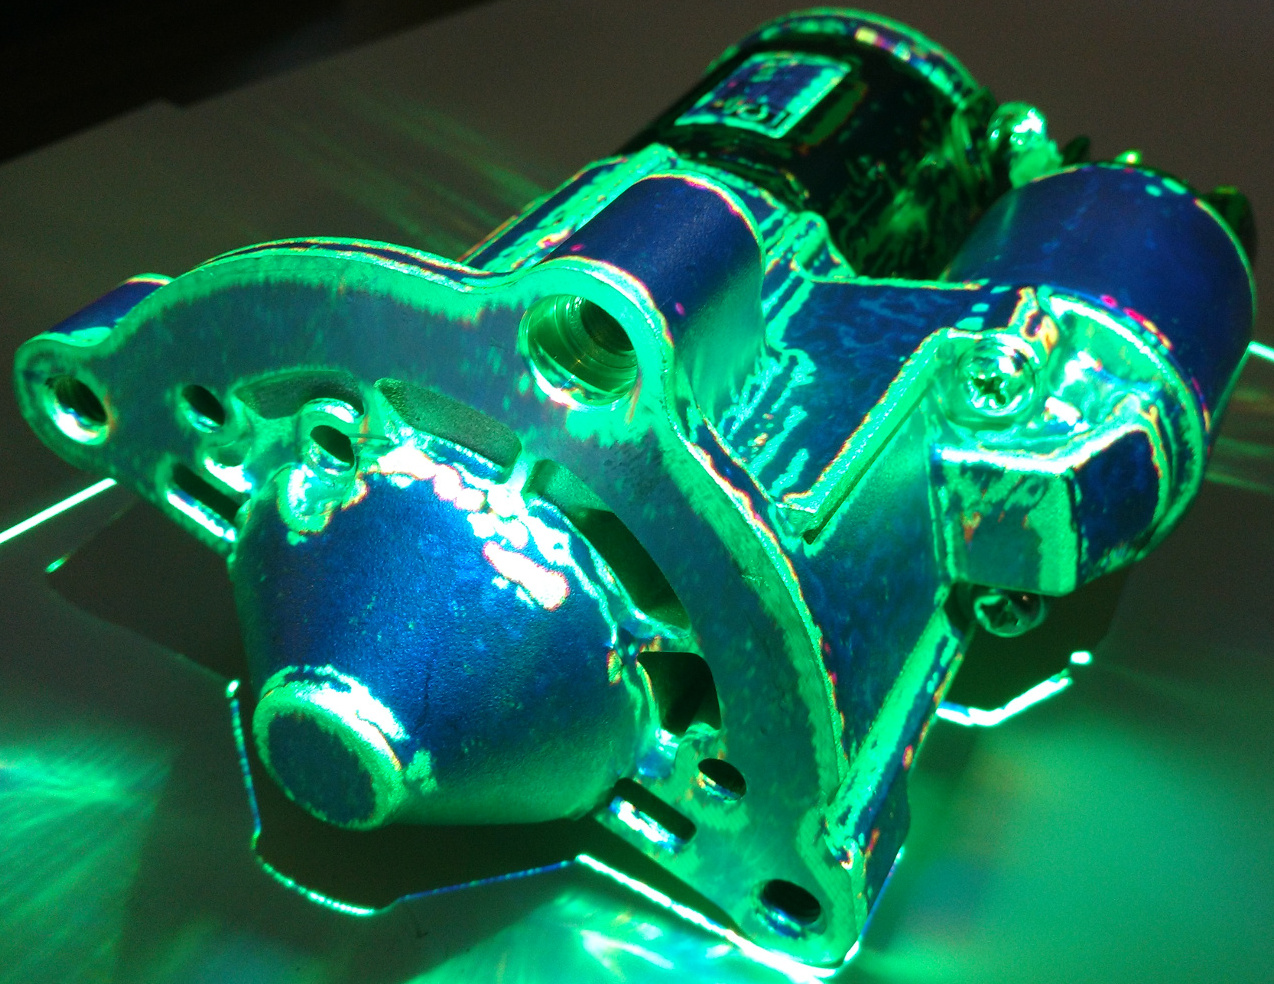
\includegraphics[height=.117\textheight]{projection-mapping-3}}
		{\caption{Projection of the outline of the reconstructed 3D model after 6 DoF pose estimation}\label{fig:projection-mapping-3}}
	\end{floatrow}
\end{figure}
